\documentclass[a4paper,8pt]{jsarticle}
%\documentclass[a4paper,10pt]{jsbook}

\usepackage[dvipdfmx]{graphicx, color}
%\usepackage{folha}
\graphicspath{{image/}}

\usepackage{color}
\usepackage{array}
\usepackage{longtable}
\usepackage{alltt}
\usepackage{graphics}
\usepackage{vpp-nms}
%\usepackage{vpp}
\usepackage{makeidx}

\usepackage{colortbl}

\usepackage[dvipdfmx,bookmarks=true,bookmarksnumbered=true,colorlinks,plainpages=true]{hyperref}


%\AtBeginDvi{\special{pdf:tounicode 90ms-RKSJ-UCS2}}
\AtBeginDvi{\special{pdf:tounicode EUC-UCS2}}


\definecolor{covered}{rgb}{0,0,0}      %black
\definecolor{not-covered}{rgb}{1,0,0}  %red

\setcounter{secnumdepth}{6}
\makeatletter
\renewcommand{\paragraph}{\@startsection{paragraph}{4}{\z@}%
  {1.5\Cvs \@plus.5\Cdp \@minus.2\Cdp}%
  {.5\Cvs \@plus.3\Cdp}%
  {\reset@font\normalsize\bfseries}}
\makeatother

\renewcommand{\sf}{\sffamily \color{blue}}

\newcommand{\syou}{\texttt{<}}
\newcommand{\dai}{\texttt{>}}

%\include{Title}

%\pagestyle{empty}
\usepackage{fancyhdr}
\usepackage{lastpage} 
  \pagestyle{fancy} 
   \let\origtitle\title 
  \renewcommand{\title}[1]{\lfoot{#1}\origtitle{#1}}

  \rfoot{\today}
  \rhead{[\ \scshape\oldstylenums{\thepage}\ / %
      \scshape\oldstylenums{\pageref{LastPage}}\ ]}
  \cfoot{}


\begin{document}

% the title page
\title{入退出管理システム:ガードコマンドと黒板によるモデルの考察}
\author{佐原 伸\\\\
タオベアーズ\\
}
%\institute{\pgldk \and \chessnl}
\date{\mbox{}}
\maketitle

%\TaoReport{ガードコマンド・モデル}{\today}{タオベアーズ}{佐原伸}
%\setlength{\baselineskip}{12pt plus .1pt}
%\tolerance 10000
\tableofcontents
%\thispagestyle{empty} 

\newpage

\section {ガードコマンドと黒板によるモデルの概要}
\label{abstract}
入退出管理システムを、状態遷移マシンが並行に動作するシステムとして記述するにあたって、
ガードコマンドと黒板を使ったモデルとして記述することにより、
仕様を逐次的に記述し検証しようというのが、
今回のモデル化のアイデアである。

基本的な振る舞いを、図\ref{fig:seqDiagram}のシーケンス図に示した、
ここで、テストケース・オブジェクトは、要求性質を検査する回帰テストケースの一つであるとともに、
入退出管理システムの外部環境や現在時間を管理し、
仕様実行のために、必要な回数だけdoOneCycleメッセージをスケジューラ・オブジェクトに送る。

ひとつのdoOneCycleが終了すると、並行実行の一つのサイクルが終了する。

スケジューラは、すべてのガードコマンドに順次checkメッセージを送ることによって、
各ガードコマンドが必要な動作を行うことを促す。

各ガードコマンドは、システムに一つしかない大域黒板から必要な黒板属性DB
\footnote{DBは、利用者がどこにいるかなどの情報を写像で持っている。}
を得てガード条件をチェックし、
ガード条件がtrueであれば、必要な動作を行う。
動作の結果は、各ガードコマンド毎に持っている局所黒板の更新黒板属性DB
\footnote{黒板属性DBに直接設定すると、各ガードコマンド動作結果により副作用が起こり得るため、更新された属性だけを持つ。}
に設定する。

スケジューラは、次に、すべてのガードコマンドに順次updateメッセージを送ることによって、
各ガードコマンドが局所黒板に設定した属性を、大域黒板に反映するよう促す。

各ガードコマンドは、局所黒板の更新黒板属性DBを得て、大域黒板の黒板属性DBに設定する。

\begin{figure}[h]
	\centering
	{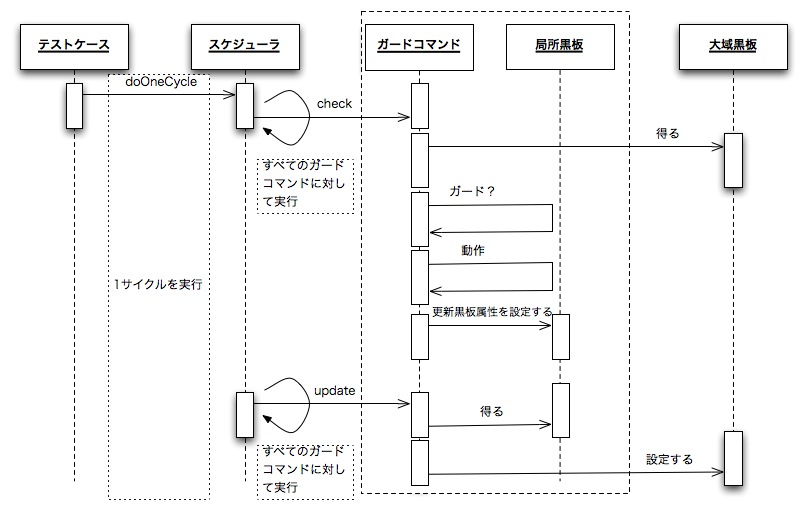
\includegraphics[width=50zw, height=40zw, keepaspectratio, bb=0 0 400 300]{image/SeqDiagram.jpg}}
	\caption{本フレームワークのシーケンス図}
	\label{fig:seqDiagram}
	\index{ふれーむわーくのしーけんすす}
\end{figure}


今回のモデル化では、仕様の変更、再利用、保守などを容易に行えるように、
仕様を図\ref{fig:hierarchie}に示す階層に従って記述した。

\begin{figure}[h]
	\centering
	{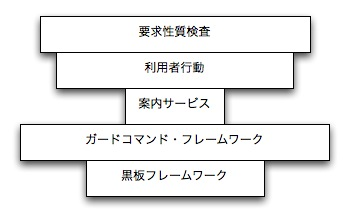
\includegraphics[width=35zw, height=40zw, keepaspectratio, bb=0 0 600 300]{image/hierarchies.jpg}}
	\caption{モデル記述の階層}
	\label{fig:hierarchie}
	\index{もてるきしゆつのかいそう}
\end{figure}

以下に、下位階層から概要を説明する。

\subsection{黒板フレームワーク}
黒板フレームワークは、黒板クラス
\footnote{以下、クラスとそのインスタンス・オブジェクトの区別は、特に必要ない限り記述しない。}
一つからなる。
黒板は、並行処理仕様を擬似的に記述するため、ガードコマンドから参照および更新される属性を持つ。

黒板には、システム全体で一つしかない大域黒板と、各ガードコマンド毎に持つ局所黒板がある。

黒板は、本来の属性を持つ黒板属性DBと、更新時の副作用を避けるために持っている更新黒板属性DBを持つ。
黒板属性DBは、すべてのガードコマンドの処理が終わるまで更新されない黒板属性DBである。
更新黒板属性DBは、各ガードコマンドが更新する黒板属性DBである。

さらに、各黒板属性は、
実際の利用者居場所DB, 仮想世界利用者居場所DB、ドアDB、
案内表示DB、ID端末DB、IDカードDB、センサー DB、タッチパネルDBを持つ。

黒板は、上記の属性を得たり、設定する操作を持っている。
また、黒板は「実際と仮想の利用者居場所が等しい」かどうか判定したり、
「データの重複がない」かを判定するといった、
要求性質の検証や仕様の検証用の操作を持つ。

\subsection{ガードコマンド・フレームワーク}
ガードコマンド・フレームワークは、
ガードコマンドの種類だけクラスが存在し、各ガードコマンド・クラスのインスタンスも通常複数存在する。

各各ガードコマンドは、checkとupdateの2つの操作を持ち、

check操作は、以下の部分からできている。

\begin{itemize}
	\item 大域黒板から黒板属性DBを得る
	\item ガード条件を判定する
	\item 対応する動作を行う
	\item 局所黒板の更新黒板属性DBに設定する
\end{itemize}

update操作は、以下の部分からできている。

\begin{itemize}
	\item 局所黒板から更新黒板属性DBを得る
	\item 大域黒板の黒板属性DBに設定する
\end{itemize}

\subsection{案内サービス}
案内アルゴリズムを記述する。

今回は、ガードコマンドとして記述した。

本来は、ID認証やセンサーから得られる情報だけで構築した、
仮想世界の利用者居場所の情報から案内すべきであるが、
後述の\ref{sec:realVsVirtual}節で述べるとおり、
正しい位置情報を得ることが非常に困難であるため、
適切に案内ができないので、
実際の利用者居場所の情報から案内を作成している。

\subsection{利用者行動}
ガードコマンド内部の動作
\footnote{VDM++\cite{CSK2007PP}の関数あるいは操作呼び出しと代入文で記述した。}
として記述した。

\subsection{要求性質検査}
回帰テストケースで、黒板クラスで定義した「実際と仮想の利用者居場所が等しい」関数と、「実際と仮想の利用者居場所を比較表示する」操作で要求性質を呼び出すことにより検査する。

\newpage

\section{ガードコマンドと黒板によるモデル化の感想}
\subsection {本フレームワークの利点}
本フレームワークを使用した結果、各ガードコマンドによるガード条件の比較と、対応する動作の記述は、
比較的単純で理解しやすく、検証しやすい。

また、当初もくろみ通り、仕様の変更を行った場合の変更余波が小さいことを実感した。

逐次型で並行処理モデルを記述できるため、同様の問題について筆者が過去に行った、
他の手法(\ref{sec:otherMethod}参照)に比べ検証が簡単である。

さらに、VDM++を使用することにより、事前条件と事後条件のチェックが可能になり、モデルの問題点を早期に発見できた
(\ref{subsec:prePost}参照)。

\subsection {実際の利用者居場所と仮想世界の利用者居場所について}
\label{sec:realVsVirtual}
センサーやID認証によって、仮想世界の利用者居場所情報を得ることを試みたが、
場所内に利用者が複数いる場合、センサー情報だけでは、誰がどこにいるかを確定することは非常に難しく、
実際に役立つのはID認証の情報だけであり、
実際の利用者居場所と仮想世界の利用者居場所の乖離がすぐに大きくなってしまった。

そのため、現在のモデルでは、案内アルゴリズムは、実際の利用者居場所から作成している。
これを、仮想世界の利用者居場所情報を元に行うと、ほぼ意味のない動きをしてしまうことが分かった。

\subsection {他の方法との比較}
\label{sec:otherMethod}
筆者が過去に行った「状態遷移マシンが並行に動作するシステム」のモデル化と今回の方式の比較を述べる。

\subsubsection{VICE\cite{CSKVICE}を使用したACSTAMモデルとの比較}
VDM++を非同期並行処理が記述できるように拡張したVICEを使用し、
(有)デザイナーズデンの酒匂寛氏が作成したACSTAMと呼ぶフレームワークを使ってモデル化を行ったが、
事前・事後条件による検証(\ref{sec:validation}節参照)は、使用できるものの、
実行テストでは、テキスト・ファイルに出力されるログをレビューしての検証しか行えず、
パラメータを少し変更するだけで、ログの内容が大きく変わり、
ある程度大きなモデルになると、検証が非常に困難になった。

仕様記述自体は、フレームワークが用意している状態遷移マシンのサブクラスとして、
例題を模倣して記述すればよいので本フレームワークと同様記述しやすい。


\subsubsection{プライオリティ・キューとイベントによる割込処理によるモデルとの比較}
このモデルは、まだある程度試行しただけで、完全なモデル化は行っていないが、
一つの状態遷移マシンを実行するプロセス(あるいはスレッド)のプライオリティキューとイベンによるト割込処理を組み合わせ、
逐次処理で「状態遷移マシンが並行に動作するシステム」を記述しようとするもので、
Zによる同様のモデル化\cite{Craig2007}も行われている。

この形のモデル化を、強い型付けの静的な言語であるVDM++で行う場合、
プロセス内で処理を実行中に割込が発生し、他のプロセスに制御が移ることは、素直にモデル化できない。

そこで、
\begin{enumerate}
	\item プライオリティ・キューとイベントによる割込処理によるプロセスの制御を記述するモデルと、
	\item 各プロセス内の処理を記述するモデル
\end{enumerate}
を別々に作らなければならず、
両モデルを、レビュー以外で統一的に検証することができない。

1.の制御方式を記述し、検証するには便利だが、
アプリケーション仕様ともいうべき2.の記述・検証には向いていないと言える。

\newpage

\section {validation方法について}
\label{sec:validation}
本モデルの検証とvalidationは下記の方法で行った。

\begin{itemize}
	\item 実行テスト
	\item 事前・事後条件
	\item 証明課題
\end{itemize}


\subsection {実行テスト}
VDM++の標準の検証手段である実行テストで、検証とvalidationを行った。
テストケースはVDM++で記述し、オランダ・チェス社のMarcel Verhoef氏が作成した回帰テスト・ライブラリを使用して、
あらかじめ設定した検証結果と実行テストの結果が一致するかを見た。

また、実行途中の重要情報は、標準出力にログとして表示し、意図したとおりの実行がなされているかを確認した。

VDM++仕様のコードカバレージは90\%以上を達成した。

\subsubsection{デバッグの工夫}
特に利用者クラスには「s前にいた場所」「s作成者名」という2つのインスタンス変数を持たせ、
ある利用者オブジェクトをどのオブジェクトが作成し、前にいた場所がどこかを確認しやすいようにした。
これにより、仕様のミスをかなり検出できるようになった。

\subsection {事前・事後条件}
\label{subsec:prePost}
主要な操作と関数には事前条件あるいは事後条件を記述し、
テスト実行時にこれら条件を検査することで、
仕様のミスを早期に発見できるようにした。

例えば、下記のVDM++ソースは、黒板に属性を設定する操作であるが、
ここで、事前・事後条件の双方で、オブジェクト参照による問題(\ref{subsec:objref}参照)から、DBに「IDの重複がある」ことを検出し、
どのような場合に起こるかの検出を容易にした。

\begin{verbatim}
public 設定する  : オブジェクト型 * DB ==> ()
設定する(aオブジェクト型, a追加DB) == (
  cases aオブジェクト型 :
    (mk_token("実際の利用者居場所")), (mk_token("仮想世界利用者居場所"))		->
      s黒板属性DB(aオブジェクト型) := 利用者居場所DBから削除する(s黒板属性DB(aオブジェクト型), a追加DB),
    (mk_token("ドア"))	-> 
      s黒板属性DB(aオブジェクト型) := ドアDBから削除する(s黒板属性DB(aオブジェクト型), a追加DB),
    (mk_token("案内表示")), (mk_token("ID端末")), (mk_token("IDカード ")), (mk_token("タッチパネル")), (mk_token("センサー"))	->
      s黒板属性DB(aオブジェクト型) := DBから削除する(s黒板属性DB(aオブジェクト型), a追加DB),
    others	->
      s黒板属性DB(aオブジェクト型) := (dom a追加DB) <-: s黒板属性DB(aオブジェクト型)
  end;
  s黒板属性DB(aオブジェクト型) := s黒板属性DB(aオブジェクト型) ++ a追加DB;
  skip
)
pre
  let wDB = s黒板属性DB(aオブジェクト型) in
  aオブジェクト型 in set dom s黒板属性DB and
  cases aオブジェクト型 :
  (mk_token("実際の利用者居場所")), (mk_token("仮想世界利用者居場所"))		->
    利用者IDの重複がない(wDB),
  others	->
    IDの重複がない(wDB)
  end
post
  let wDB = s黒板属性DB(aオブジェクト型) in
  cases aオブジェクト型 :
  (mk_token("実際の利用者居場所")), (mk_token("仮想世界利用者居場所"))		->
    利用者IDの重複がない(wDB),
  others	->
    IDの重複がない(wDB)
  end;
\end{verbatim}

\subsection {証明課題}
証明課題を生成しレビューすることで、
下記\ref{subusubsec:notNil}節以下で説明するように、仕様の誤りをいくつか検出した。

これらの証明課題以外にも、いくつかのタイプの証明課題から、
事前・事後条件を導出し、仕様中に記述した。

\subsubsection{値が空でないことや0でないこと}
\label{subusubsec:notNil}
束縛された値が空でないといった証明課題から、
不注意により、空集合にはならないはずの箇所で、
空集合になるバグをいくつか発見できた。

\paragraph{空である場合のチェック}
下記の例では、証明課題をレビューすることで、利用者集合が空であるケースを見落としていた
仕様のミスを検出した。

\begin{verbatim}
(forall a利用者集合 : set of 利用者 &
a利用者集合 <> {} =>
 (exists w次の利用者 in set a利用者集合 &
(forall w利用者 in set a利用者集合 &
w次の利用者.s到着時間 <= w利用者.s到着時間)))
  \end{verbatim}
  
  修正後のVDM++ソースは以下の通りである。
  
\begin{verbatim}
static public 到着時間が一番早い利用者を選ぶ : set of 利用者 -> 利用者
到着時間が一番早い利用者を選ぶ(a利用者集合) == 
  let w次の利用者 in set a利用者集合 be st
    forall w利用者 in set a利用者集合 & w次の利用者.s到着時間 <= w利用者.s到着時間
  in
  w次の利用者
pre
  a利用者集合 <> {}
post
  forall w利用者 in set a利用者集合 & RESULT.s到着時間 <= w利用者.s到着時間;
\end{verbatim}

\paragraph{分母が0である場合のチェック}
\label{para:0divide}
下記の証明課題をレビューすることで、分母が0になってしまうケースを見落としていたバグを発見できた
\footnote{このケースは、VDMの別の処理系Overture Tool(http://www.overturetool.org/twiki/bin/view)で発見した。
現在のVDMToolsは過去にはこの類の証明課題を生成していたが、今は。何故か表示しない。}。

\begin{verbatim}
(not (s躊躇する最大時間 = 0) => s躊躇する最大時間 <> 0)
\end{verbatim}

修正後のVDM++ソースは以下の通りである。

\begin{verbatim}
public 移動する気になった時間である : () ==> bool
移動する気になった時間である() == 
  def w乱数 = MATH`rand(s躊躇する最大時間);
    w時間の乱れ = 
      if s躊躇する最大時間 = 0 then
        0
      else
        w乱数 / s躊躇する最大時間;
    w移動する気になった時間 = s躊躇する最大時間 * w時間の乱れ
  in (
  def - = 
    debug >= 9 => new IO().echo(
      "\n「移動する気になった時間である」で生成された乱数=" ^
      VDMUtil`val2seq_of_char[int](w乱数)^
      "\n"
    )
  in skip;
  return s現在時間 >=  w移動する気になった時間 + s到着時間;
)
\end{verbatim}

\subsubsection{subtypeが適切であること}
演算の中間結果が、不注意によって int でなく real になっていたことに気がつき、
影響がないかどうか、該当箇所を調べているうちに、
VDMの処理系によって結果が異なる箇所を発見することができ、
ツールの欠陥を発見できた。

具体的には、\ref{para:0divide}節と同じ下記のソースで、
「w時間の乱れ」の型がrealになっている影響を調査している内に、
rand関数の返値がVDMToolsとOverture Toolで異なることを発見し、
Overture Toolのバグを検出した。

\begin{verbatim}
public 移動する気になった時間である : () ==> bool
移動する気になった時間である() == 
  def w乱数 = MATH`rand(s躊躇する最大時間);
    w時間の乱れ = 
      if s躊躇する最大時間 = 0 then
        0
      else
        w乱数 / s躊躇する最大時間;
    w移動する気になった時間 = s躊躇する最大時間 * w時間の乱れ
  in (
  以下、省略...
\end{verbatim}

\subsubsection{map application}
写像のdomein側の値が不適切であるケースを発見した。

\paragraph{写像の適用}
下記の証明課題をレビューすることで、
該当の操作に、証明課題と同じ事前条件が必要なことに気づいた。

\begin{verbatim}
a居場所ID in set dom s移動可能場所集合
\end{verbatim}

\begin{verbatim}
public 移動可能な次の場所IDを得る : 利用者のいる場所DB * 場所ID ==> [場所ID]
移動可能な次の場所IDを得る(a利用者のいる場所DB, a居場所ID) == (
  for all w次の場所ID候補 in set s移動可能場所集合(a居場所ID) do
    if 利用者が移動可能である(a利用者のいる場所DB, w次の場所ID候補) then
      return w次の場所ID候補
    else
      skip;
  return nil
)
pre
  a居場所ID in set dom s移動可能場所集合;
\end{verbatim}

\newpage

\section {VDMコーディング上のコツ}
\subsection {オブジェクト参照の問題}
\label{subsec:objref}
本モデルでは、黒板中に持つ属性を写像で保持し、そのドメインあるいは値域にオブジェクトを使用している場合が多い。

この場合、
黒板属性中のオブジェクト内容を変更して更新黒板属性としても、
オブジェクト参照のため元の黒板属性の内容も書き換わってしまう。

このため、新たなオブジェクトを作成して、黒板属性中のオブジェクト内容をコピーすると、
写像中では異なるオブジェクトとなるため、削除してから新規
に追加する形で更新しなければならない。

ところが、旧黒板の内容を参照して削除しようとすると、
2つのガードコマンドが同じ黒板属性を同じタイミングで更新する場合、
update時に最初のガードコマンドが削除・更新したオブジェクトを、
2つめのガードコマンドは削除前のオブジェクトを参照して削除しようとするため、
削除できずに同じID(例えば利用者ID)を持つオブジェクトを2つ作ってしまう。

そこで、本モデルでは、各オブジェクトのID
\footnote{言語処理系が自動付与するオブジェクトIDでなく、仕様記述者が設定するID}
を設定し、
写像中のオブジェクトを更新する場合、
check操作中で、
下記\ref{subsubsection:copy}節のように、
写像中のオブジェクトをコピーして、
新たに同じ値を持ったオブジェクトを作成して属性を更新し、
update操作から呼び出す「設定する」操作で、
下記\ref{subsubsection:deleteAndAppend}節のように、
写像中のオブジェクトを削除(\ref{subsec:delete}節を参照)してから、
新しいオブジェクトを追加するようにした。

\subsubsection{オブジェクトのコピー}
\label{subsubsection:copy}
\begin{verbatim}
public check : 黒板 ==> ()
check (a大域黒板) == (
  ...
  dcl w更新ID端末 : ID端末 := wID端末.コピーする(w位置);
  dcl w更新開くべきドア : ドア := w開くべきドア.コピーする(mk_(f, t));
  w更新開くべきドア.解錠する();
  w更新ID端末.利用可能にする();
  s局所黒板.更新黒板属性を設定する(mk_token("ドア"), {mk_(f, t) |-> w更新開くべきドア});
  s局所黒板.更新黒板属性を設定する(mk_token("ID端末"), {w更新ID端末.位置を得る() |-> w更新ID端末});
  ...
\end{verbatim}

\subsubsection{オブジェクトの削除と追加}
\label{subsubsection:deleteAndAppend}
\begin{verbatim}
public 設定する  : オブジェクト型 * DB ==> ()
設定する(aオブジェクト型, a追加DB) == (
  cases aオブジェクト型 :
  (mk_token("実際の利用者居場所")), (mk_token("仮想世界利用者居場所"))		->
    s黒板属性DB(aオブジェクト型) := 利用者居場所DBから削除する(s黒板属性DB(aオブジェクト型), a追加DB),
  (mk_token("ドア"))	-> 
    s黒板属性DB(aオブジェクト型) := ドアDBから削除する(s黒板属性DB(aオブジェクト型), a追加DB),
  (mk_token("案内表示")), (mk_token("ID端末")), (mk_token("IDカード ")), 
  (mk_token("タッチパネル")), (mk_token("センサー"))	->
    s黒板属性DB(aオブジェクト型) := DBから削除する(s黒板属性DB(aオブジェクト型), a追加DB),
  others	->
    s黒板属性DB(aオブジェクト型) := (dom a追加DB) <-: s黒板属性DB(aオブジェクト型)
  end;
  s黒板属性DB(aオブジェクト型) := s黒板属性DB(aオブジェクト型) ++ a追加DB;
)
\end{verbatim}


この方式の欠点は、
各クラスに「コピーする」操作を作成しなければならない点と、
各オブジェクトによって、写像からの具体的削除方法が異なるため、
仕様の行数がやや長くなる点であるが、本モデルでは、できるだけ共通化するようにし、
実際の利用者居場所DBとドアDBおよびその他のDBの3パターンに集約できた。

\subsection {写像からの削除方法}
\label{subsec:delete}
写像中のオブジェクトの削除を定義域削減($ <-:$)演算子で行うと、
同じオブジェクトID(VDM++処理系が付与するID)を持つオブジェクトを等しいと判断するため、
新たに作成した
同じID(例えば利用者ID)を持つオブジェクトを異なるオブジェクトと判断し、
同じIDのオブジェクトが写像中に2つ作成されてしまう。

そこで、\ref{subsubsection:deleteFromDB}節のように、オブジェクトのID集合と削除すべきIDの集合から、
削除後のID集合を求め、
次に、そのIDを持つ集合を求め、
さらに、値域限定演算子を使って、削除後の写像を求める。

\subsubsection{DBからの削除}
\label{subsubsection:deleteFromDB}
\begin{verbatim}
public DBから削除する : 場所関連DB * 場所関連DB -> 場所関連DB
DBから削除する(aDB, a削除DB) == 
  if aDB <> {|->} then
    let w集合 = rng aDB,
      wID集合 = {w.IDを得る() | w in set w集合},
      w削除集合 = rng a削除DB,
      w削除ID集合 = {w.IDを得る() | w in set w削除集合},
      w削除後ID集合 = wID集合 \ w削除ID集合,
      w削除後集合 = {w | w in set w集合 & w.IDを得る() in set w削除後ID集合}
    in
    aDB :> w削除後集合
  else
    aDB;
\end{verbatim}


\subsection {今回のモデル実装上の問題点}
黒板属性を写像とオブジェクトで表現したため、上記\ref{subsec:objref}節と\ref{subsec:delete}節の問題が発生した。

そこで、黒板の属性を、写像とオブジェクトでなく、集合とレコードで表すことが考えられる。
この方式は、今回は採用できなかったが、他のアプリケーションでは成功したことがあり、
今後研究する価値があると考える。

%\begin{thebibliography}{9}
\section{参考文献等}

\bibliographystyle{jplain}
%\bibliography{/Users/sahara/svnw/sahara}
\bibliography{/Users/sahara/Dropbox/bib/saharaUTF8}

%\end{thebibliography}

%\newpage
%\addcontentsline{toc}{section}{Index}
%\printindex

\end{document}
